\documentclass[authoryear]{elsarticle}

%\pagenumbering{gobble}

\usepackage{threeparttable}
\usepackage{caption} 
\captionsetup[table]{skip=0pt}

\makeatletter
\def\ps@pprintTitle{%
\let\@oddhead\@empty
\let\@evenhead\@empty
\def\@oddfoot{}%
\let\@evenfoot\@oddfoot}
\makeatother

\setlength\arraycolsep{2pt}
\setlength{\parskip}{1ex plus 0.5ex minus 0.2ex}
\usepackage{graphicx}

\usepackage{amsfonts}
\usepackage{multirow}
\usepackage{comment}

%hello there
%\usepackage{chicago}
\bibliographystyle{chicago}



\newcommand{\eps}{\epsilon}
\newcommand{\var}{{\rm var}}
\newcommand{\cov}{{\rm cov}}
\newcommand{\nid}{{\rm NID}}
\newcommand{\diag}{{\rm diag}}
\newcommand{\E}{{\mathrm E}}
\newcommand{\R}{{\mathrm R}}
\newcommand{\RD}{{\tilde{\mathrm R}}}
\newcommand{\Q}{{\mathrm Q}}
\newcommand{\U}{{\mathrm U}}
\newcommand{\Ex}{{\cal E}}
\newcommand{\cor}{\mathrm{cor}}
\newcommand{\tr}{\mathrm{tr}}
\newcommand{\e}{\mathrm{e}}
\newcommand{\de}{\mathrm{d}}
\newcommand{\p}{\mathrm{P}}
\newcommand{\Ln}{\mathrm{Ln}}
\newcommand{\sign}{\mathrm{sign}}
\newcommand{\sref}[1]{Section \ref{#1}}


\newcommand{\ra}{\varrho}

\newcommand{\minn}{\mathrm{min}_n}
\newcommand{\maxn}{\mathrm{max}_n}


\newcommand{\cq}{\ ,\quad }
\newcommand{\qq}{\quad \Rightarrow \quad}
\newcommand{\oq}{\quad \Leftarrow \quad}
\newcommand{\eq}{\quad \Leftrightarrow \quad}

\newcommand{\be}[1]{\begin{equation}\label{#1}}
\newcommand{\ee}{\end{equation}}

\newcommand{\ppo}[1]{|{#1}|^+}

\newcommand{\ssection}[1]{%
  \section[#1]{\textbf{\uppercase{#1}}}}
\newcommand{\ssubsection}[1]{%
  \subsection[#1]{\normalfont\textbf{#1}}}


%\renewcommand{\labelenumi}{(\roman{enumi})}

\newcommand{\eref}[1]{(\ref{#1})}
\newcommand{\fref}[1]{Figure \ref{#1}}
\newcommand{\tref}[1]{Table \ref{#1}}
\newcommand{\aref}[1]{\ref{#1}}



\newcommand{\bi}{\begin{itemize}}
\renewcommand{\i}{\item}
\newcommand{\ei}{\end{itemize}}


\newcommand{\sr}{\ensuremath{\mathrm{SRISK}}}
\newcommand{\br}{\ensuremath{\mathrm{BRISK}}}
\newcommand{\pr}{\ensuremath{\mathrm{PRISK}}}

\newcommand{\Es}{\ensuremath{\widetilde\E}}



\newcommand{\es}{{\mathrm{ES}}}
\newcommand{\ses}{{\mathrm{SES}}}


\begin{document}



\begin{frontmatter}



\title{An early warning tool for measuring the build up of systemic risks in banks and financial systems}

  \author{Piet de Jong\footnote{
    The authors gratefully acknowledge the financial and other support from the Centre of International Financial Regulation (CIFR).}\hspace{.2cm}\\
    Department of Applied Finance and Actuarial Studies, Macquarie University\\
    and\\
    Weihao Choo\\
    Department of Applied Finance and Actuarial Studies, Macquarie University
        and \\
    Geoffrey Loudon\\
    Department of Applied Finance and Actuarial Studies, Macquarie University\\}



\begin{abstract}
This paper develops, analyses and implements an early warning tool for  systemic risk in banks and financial entities. The tool is based on a refined approach to stress testing. Calculations performed on Australian bank data are shown to predict past distres. Risk is measured as  a function of expected capital shortfall in individual firms. A simple model of regulatory capital is assumed. Systemic risk is shown to be driven by the size and leverage of balance sheets and interdependence between firms.  Firm balance sheets are modelled using publicly available information and assumed to depend on market returns. Model refinements using more comprehensive information and practical implementation are also discussed.

\end{abstract}

\end{frontmatter}




\section{Systemic risk and stress testing}\label{sreview}
%This section gives an overview of the industry view of systemic risk and stress testing

Systemic risk is the risk of a system-wide loss or failure, and is inherent in the financial industry due to firms with large, leveraged and interrelated balance sheets. The impact of systemic risk was felt
 during the 2008 global financial crisis (GFC) where the housing market downturn and Lehman Brothers failure triggered crisis in other financial firms and the global economy. The crisis was caused, amongst  other factors, by financial firms relying on one another and the state of the economy to sustain highly leveraged financial positions via the use of derivatives. The Lehman Brothers  failure directly or indirectly affected others. See \cite{kolb2010lessons} for a discussion of the 2008 global financial crisis.


Drivers of systemic risk are:
\begin{enumerate}

\i Financial dependence between firms
\i Dependence of individual firms  on common macroeconomic factors and market conditions
\i Proportionally large balance sheets of key  individual firms
\i High leverage with debt  many times the value of net assets

\end{enumerate}

Industry stress tests for banks conducted in 2010, 2012 and 2014 by the Australian Prudential Regulation Authority (APRA), and a recent exercise for life insurers, demonstrate the regulator's concern with the presence and extent of systemic risk in the financial industry. Stress testing examines the impact of a set of adverse assumptions or scenarios on the financial position of a firm. For the most recent banking stress test, interest rates and unemployment rates were assumed to increase over a prolonged period, resulting in a series of losses particularly from credit defaults.


Industry stress testing is an effective systemic risk measurement tool for two reasons. Firstly, balance sheets at face value do not apparently indicate the level of systemic risk. Two balance sheets may look similar but diverge significantly when a stress is applied, due to differences in business profile or the nature of assets and liabilities held. For example the loan portfolio of a bank may be diversified across Australia and overseas, whereas the same for another bank may be concentrated in a particular state or industry in Australia. A systemic stress is likely to have a far larger impact on the latter. Secondly, applying common adverse assumptions to all firms, rather than having firms select their own assumptions, leads to a realistic impact analysis of a market downturn.


Apart from industry stress testing, APRA imposes a set of prudential standards for financial firms to manage their solvency. Relevant standards relate to capital management: APS 110, GPS 110 and LPS 110 for banks, general insurers and life insurers, respectively, and risk management: CPS 220 for all financial firms. Specific requirements which are relevant to this paper are:
\bi

\i Using stress and scenario testing to identify and manage key risks. This is in addition to above industry stress tests.

\i Setting a risk appetite statement including a limit on the probability or extent of default, and monitoring the adherence to the limit.

\i Capital requirements which reflect the volatility of assets and liabilities held and their mismatch.

\ei

Financial markets are increasingly globalised with large firms having a presence in most major markets. Managing systemic risk globally has led to the identification and additional regulation of systemically important banks and insurers. These banks and insurers are identified using a similar set of  factors as those described above: the size of the balance sheet, extent of leverage, links with the financial market, and the impact of stressed financial conditions.





\section{Contributions of this paper}
%This section highlights contributions of the paper and introduces the 8 banks used

This paper proposes and develops an approach to assess the extent of systemic risk in the market as a whole and in individual firms.  The approach models  the impact of a stress on default risk and expected capital shortfall. Specific contributions are:
\bi
\i The notion of systemic risk is formalised as increases in expected capital shortfall under stress.

\i Stress testing is enhanced by considering all possible scenarios rather than one or more specific scenarios.

\i Baseline risk is present in the system even without stress and is again based on expected capital shortfall.

\i A forward looking tool is proposed to continuously monitor baseline and systemic risks in the entire market and firm contributions.
\ei
Systemic risk defined in this paper reaffirms and formalises key drivers listed in the previous section: size, leverage and interdependence between balance sheets of individual firms. Calculations are performed on past Australian bank data which includes the 2008 GFC. Results show heightened systemic risk in the lead up to, and during, the 2008 GFC. In addition the extent of systemic risk at present is significantly higher compared to levels 10 or 20 years ago, arguably due to not only persistent turbulence in global financial markets but also increased connectivity between firms.


Throughout this paper a one--factor model of regulatory capital requirements is assumed across all firms. This assumption removes complications of capital requirements in practice which vary between firms and across banks, general insurers and life insurers. These complications are not central to the development of this paper. Refining the model to reflect capital requirements in practice leads to straightforward modifications of results in this paper.


Calculations of systemic risk in this paper enhance the recent SRISK approach in \cite{brownlees2015} and are akin to default put options discussed in \citet{merton1977analytic}, \citet{doherty1986price}, \citet{cummins1988risk}, \citet{myers2001capital} and \citet{sherris2006solvency}. In addition the refined stress testing approach follows the concept of probability distortion \citep{wang2000class}, weighted average loss \citep{choo2009loss} and yields covariance based results similar to those in \cite{ruhm2003risk} and \cite{choo2010determining}.


To demonstrate the nature and usefulness of the proposed framework, the methodology is applied to eight Australian banks detailed in \tref{eightbanks} using publicly available daily financial data spanning 3 April 2000 through to 1 December 2014.  Stock prices, adjusted for dividends, are plotted in \fref{prices}.  The data is described in detail in \aref{data}.  Stock prices are multiplied by the number of shares to derive total equity. Total debt for each firm at each point of time are derived from annual accounting reports.

\begin{table}[htbp]
\label{banks}\caption{Major and minor Australian banks}\label{eightbanks}
\begin{center}
\begin{tabular}{l|l||l|l}
\hline
 \multicolumn{2}{c||}{Major}& \multicolumn{2}{c}{Minor}\\
 \hline
CBA & Commonwealth   & MQG  & Macquarie \\
ANZ  & Australia \& New Zealand  & BOQ  &  Queensland\\
NAB  & National Australia  & BEN & Bendigo and Adelaide \\
WBC  & Westpac & ABA & Auswide \\
\hline
\end{tabular}
\end{center}
\end{table}

\begin{figure}[htbp]
\begin{center}
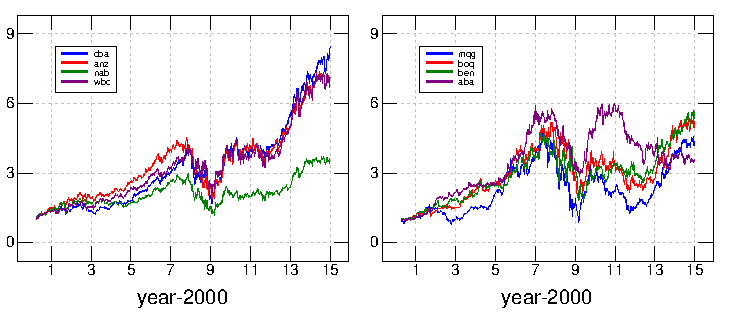
\includegraphics{figures/prices.pdf}
\caption{Stock  prices of four major (left panel) and four minor (right panel) Australian banks from early 2000 through to the end of 2014.  Price series normalised to start at 1.}
\label{prices}
\end{center}
\end{figure}

Remaining sections are structured as follows. Sections  \aref{s_capmodel} and \aref{s_expshort} outline a simple model of current and future capital shortfall based on a one factor model of regulatory capital. Section \aref{s_forward} describes how future expected capital shortfall can be monitored by modelling balance sheets based on available information. The model is applied to remaining developments of this paper. Sections \aref{s_st}, \aref{s_sfactor}, \aref{s_extend} and \aref{s_stmarket}  discuss the shortcomings of current stress testing approaches and put forward enhancements which form the definition of systemic risk. Section \aref{s_formal} formalises the risk framework proposed in this paper by separating baseline risk and systemic risk and monitoring firm contributions and market totals. Further illustrations using Australian bank data are provided in section \aref{s_app}. Section \aref{s_concl} concludes this paper by discussing ways to improve the risk modelling and the associated practical challenges.


\section{Regulatory capital and capital shortfall}\label{s_capmodel}
%This section introduces the simplistic model of capital shortfall


Capital shortfall of a firm is the gap between available capital and the regulatory required amount. Write $d$ and $w$ as the debt and equity of a firm at a particular point in time. Then assets are $d+w$. Suppose $0<k<1$ is the regulatory capital requirement as a proportion of assets, capturing market, credit, insurance, operational and other risks.   Then the capital shortfall is
\be{shortfall0}
 S\equiv k\times\mathrm{assets} - \mathrm{equity} = k (d+w)-w = k d\left(1-\frac{1-k}{kL}\right)\cq L\equiv \frac{d}{w} \ ,
\ee
where $L$ is the leverage.  In many cases for banks $k$  is approximately 8\%, sometimes called the ``Basel" requirement. 

A negative capital shortfall implies  there is capital surplus.   Hence the effective shortfall is  the positive part of $S$, denoted $S^+$ and  $S^+=0$  unless equity $w$ is less than the prudential fraction $k$ of assets $d+w$.

In practice there  may be additional adjustments to the prudential fraction such as those relating to intangible assets and liability surpluses. Firms usually need to maintain an equity buffer above the regulatory capital requirement and hence the true capital shortfall is higher than in \eref{shortfall0}. These adjustments are ignored to keep the model simple and tractable.

The following features of capital shortfall in \eref{shortfall0} reflect practice:
\bi

\i Shortfall $S$ increases with the prudential fraction $k$, debt $d$, and leverage $L$.


\i If  $k=1$ then $S^+=S=d$.  Further $k=0$ implies $S^+=0$.


\i $S^+$ exceeds zero if and only if $L>(1-k)/k$: leverage exceeds a threshold computed from the prudential fraction $k$.


\i As  leverage $L$ becomes large,  both $S$ and $S^+$ approach $k d$. Thus $kd$ is approximately the amount of capital required for a very highly leveraged firm.

\ei

\section{Future capital shortfall}\label{s_expshort}
%This section extends the previous section to consider future capital shortfall and its expectation

Firms and regulators are interested in future capital shortfall such as the shortfall of a bank in one month's time.   A projected shortfall, couched in terms of  probabilities, may lead to regulatory action.  If $r$ is the log--return on equity over the next period and debt $d$ stays fixed then  future leverage is $d/(\e^r w)= \e^{-r}L$ where $L$ is the current leverage.  Then the future shortfall is
\begin{equation}\label{shortfall1}
S \equiv k d  (1-\e^{r-\ell})\cq \ell\equiv \ln L + \ln\frac{k}{1-k}   \  ,
\end{equation}
where $\ell$ is called the adjusted log--leverage.   If $r=0$ then \eref{shortfall1} reduces to current shortfall.
The assumption of constant debt $d$ is reasonable if the period is small such as a month, but can be relaxed with the availability of more comprehensive data such as detailed debt or liability profiles.  

If $S$ is unknown it may be simulated based on an assumed model and appropriate scenarios.     Distributions of simulated values mimicking actual probability distributions are based on ``best estimate assumptions" which are derived from available data and judgement without deliberate bias. Stressed probability distributions  introduce deliberate conservatism or biases and are discussed later.
This paper simulates one month ahead shortfalls $S$ in \eref{shortfall1} using  a stochastic model for $r$ fitted using publicly available stock returns for Australian banks.   The aim is to provide a monthly monitoring tool for the real time assessment of risks and particularly systemic risks in each bank and the banking system as a whole. 

With $S$  as in \eref{shortfall1} write $S^+$ as the positive part of $S$ equivalent to  $kd$ times a put with strike 1.   A return $r$ less than $\ell$ implies a positive shortfall.   The put value increases  with the adjusted log--leverage   $\ell$ and the fraction margin $k$.       Volatility in the return $r$ and negative return tail risk  increase the expected put value.  

\section{Forward looking risk assesment}\label{s_forward}

Assessing future shortfall  $S$  gives a picture of the risk faced by the bank.  Regulators such as APRA are interested in real time monitoring of likely values of $S$ across  financial firms. Upward trends in $S$ or $\E(S)$ caused by heightened levels of either debt, leverage or return volatility  suggest  greater required oversight.

This section displays one month ahead simulated values of $S$ and market return  using a joint model based on daily bank and market returns.   The market return captures  a common driver of individual bank returns and individual bank shortfalls and permits the assessment of risk to individual banks of say a major overall market correction.    Aggregating shortfalls across banks  under such a scenario leads to an understanding of systemic risk.   The approach has recently been advocated in  \cite{brownlees2015} where dependencies in different firms  future rates of return  are modelled  using a daily GARCH--DCC time series model fitted using historical (relative to each month)  daily stock prices and market returns with  model parameters updated  as additional data become available.   The GARCH--DCC model  \citep{engle2002dynamic} captures shifts in return volatility over time, an important characteristic of stock returns. The GARCH--DCC model also captures the well known market phenomenon of changes in correlation between individual and overall market returns over time.    

 \fref{figCBA}   displays two snapshot outputs from  6000  simulated one month forward projected shortfall $S$ for  CBA and the return in the general market, on  two dates: the start of January 2009 and the start of December 2014.  Thus the projection is the return over the next month based on available data at the start of the month. The simulated points do not involve look--ahead bias as the model at each time point is based on the available data to that point in time. 
 
    The two panels  display very different volatility and slopes. In January 2009 both $S$ and market return distributions are highly volatile and correlated. The correlation remains strong in December 2014 but with less return volatility. These snapshots are used to compute baseline and systemic stresses discussed in subsequent sections.

Based on the available data at the two points in  time, policy makers and regulators faced entirely different projections.      The  horizontal origin line in each panel indicates the Basel limit:  an $S$ value greater than the limit leads to a Basel breach.   In the left panel there is a high likelihood that the Basel limit will be breached.  In the right panel there is no chance of a Basel breach -- the bank is ``safe" under all market scenarios.

 The black dots in each panel indicate the actual outcome after one month in both the market return and the bank shortfall \eref{shortfall0}.    In the left panel the outcome is a decline in   the market and  a shortfall $S>0$.    In the right panel there is a market downturn and a slight  increase in $S$ although $S$ remains negative.    Thus at the beginning of January  2009 CBA was projected to be far from compliance at the end of the  month while in December 2014 the one month projection suggests complete compliance.

\begin{figure}[htbp]
\begin{center}
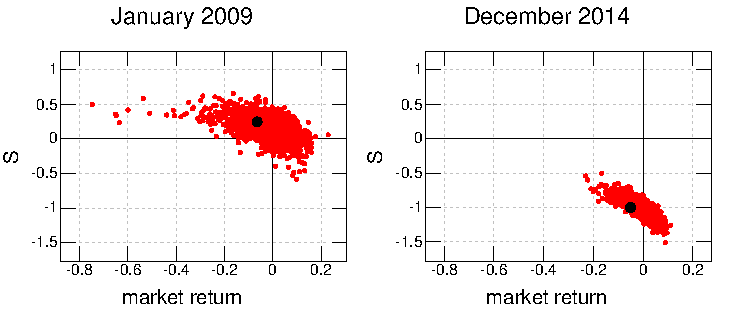
\includegraphics{figures/figCBA.pdf}
\caption{Forecast bivariate distribution of future shortfall $S$ per unit $kd$  for CBA (vertical axis) and market rate of return (horizontal axis) at start of January 2009 (left panel)  and December 2014 (right panel). Note scales in both panels are the same, the relatively large volatility in the left panel, and the left skew in the  marginal distributions.  Black dots indicate actual  outcome at the end of the month.}\label{figCBA}
\end{center}
\end{figure}

There is no look--ahead bias in the calculations:  at any point estimates are computed using a model fitted to information available at that time.  For example the $S$ distribution at the  end of August 2013 is computed using debt and leverage levels at the end of July 2013 and the probability distribution of August returns fitted using past returns up to end July.  The GARCH--DCC model is only one possible implementation and other time series models may be used if they are shown to be more appropriate.




\section{Monitoring shortfall in real time}\label{brisk}

Measures of expected future shortfall or baseline risk include
$$
\E(S) \cq \{\E(S)\}^+ \cq \E(S^+)= \p(S>0)\E(S|S>0)\ . 
$$
The first, $\E(S)$, can be positive or negative while the second and third are nonnegative.   The second measure is used in \cite{brownlees2015} to define a quantity called  SRISK.  The plus superscript denotes the ``positive part of."  The final measure $\E(S^+)$ focusses on the average of positive shortfalls and is the measure used in this study.   As indicated $\E(S^+)$ decomposes into the probability of a positive shortfall times the expected size of the shortfall given it is positive.   These two latter measures can individually be used as measures of the risk of shortfall.

This section displays the results from analyses as in the last section but now for all 8 banks listed \tref{eightbanks} and for the start of  each month,  beginning in 2003 and ending December 2014.   Simulated one month forward returns are used to calculate the normalised actual shortfalls
$
S^+/(kd)
$.
 As in \cite{brownlees2015}, $k=0.08$ while $d$ is the debt and for the given bank at the given time.  Using $S^+/(kd)$ rather than $S^+$  facilitates comparison across banks and  time.

Results are displayed in the two  panels of \fref{defaulttop} displaying baseline risk $\E(S^+)$ for the major and minor banks. The first suggestion of material expected shortfall arose with NAB  in early 2008 followed one month later by ANZ , and a further few months later by WBC  and CBA. Expected shortfall subsided shortly after 2009, however NAB 's position deteriorated again in 2011 lasting until 2013. 

\begin{figure}[htbp]
\begin{center}
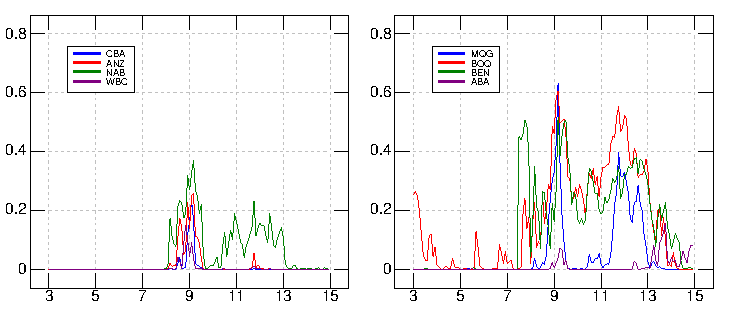
\includegraphics[width=12cm]{figures/defaulttop.pdf}
\caption{Baseline risk $\E(S_i^+)$  for   major (left panel) and  minor (right panel)  banks 2003--2014.}\label{defaulttop}
\end{center}
\end{figure}

The  panels in  \fref{defaulttop} display baseline risk: that is risk without assuming or conditioning on a stressful event.   Conditioning on such events leads to stress testing discussed in the next section.


\section{Stress testing based on single adverse event}\label{s_st}

Regulators focus on downside risk and focus on  capital shortfall $S$ or $S^+$ using conservative rather than best estimate assumptions. As discussed above, stress testing imposes adverse scenarios and is an important tool to assess systemic risk. The following  discusses standard stress testing and the next section shows a refined approach to stress testing applied to  shortfall $S$ of the  previous sections.

Common stress testing techniques, including those prescribed by APRA in its industry stress tests, focus on a single adverse scenario $\omega$ and its impact, that is the conditional expectation $\E(S|\omega)$. For example the 2014 industry stress test for banks consisted of two scenarios, one of which assumed that Australia GDP would contract by $4\%$ in 2015 and only return to positive growth in 2017. Adverse scenarios were also imposed on interest rates and unemployment during the same period.

Consider
$
\E(S| \omega)$ 
where $\omega$ is the event of  a market return less than say $-10\%$.   Thus the shortfall calculations are conditional on the basis of a substantial market correction.   In terms of \fref{figCBA} the conditioning considers all points to the left of $-10\%$ on the horizontal axis and computes the expected shortfall  or probability of shortfall  on the basis of these CBA returns.   
Measures of stress caused by stress event $\omega$   include 
$$
\E(S|\omega)-\E(S)\ ,
$$ 
that is, the  increase in the expected shortfall or proportionate increase in the probability of default. 




There are two shortcomings when focus is placed on a single scenario:
\bi
\i All other scenarios are ignored. GDP growth, interest rates, market  returns, unemployment rates and other factors take on a continuous range of values. Hence assuming that market index returns are less than $-10\%$, for example, in stress testing and assessing the financial impact ignores the possibility of other adverse scenarios.

\i Focusing on a single scenario ignores the stochastic or probabilistic nature of actual outcomes. Additionally  when various scenarios are considered, there is no coherent framework to combine the scenarios to assess the overall stress impact on each firm. Hence stress test results are scattered, impede interpretation and may make for ambiguity.
\ei

\section{Stress testing based on more than one adverse event}\label{s_extend}

With more than one possible events $\omega$ covering the range of all possible scenarios, then\footnote{The sample space of possible scenarios is assumed discrete.   If not,  sums are replaced by integrals.  Also note that the development here and below can use either $S$ or $S^+$.} 
\begin{equation}\label{stress1}
\E(S) =  \sum_\omega f(\omega) \E(S|\omega)\cq \sum_\omega f(\omega)=1\ ,
\end{equation}
where $f(\omega)$ is the probability associated with scenario $\omega$.  
Hence expected capital shortfall combines conditional expectations under various scenarios using actual probabilities. Scenarios may represent simulations from a stochastic model.   Alternatively, scenarios relate to outcomes of market or macroeconomic factors during the upcoming period such as interest rates, credit spreads, market index returns, unemployment rates, house prices, inflation and economic growth. Subsequent sections of this paper assume a single factor driving the scenarios: market index returns.

Replacing the probabilities $f(\omega)$  in \eref{stress1} by distorted probabilities $\tilde f(\omega)$ leads to the distorted expectation
\begin{equation}\label{stress2}
\widetilde \E(S) =  \sum_\omega \tilde f(\omega) \E(S|\omega)\cq \sum_\omega \tilde f(\omega)=1\ .
\end{equation}
 Distorted  probabilities usually magnify the likelihood of adverse scenarios and diminish the likelihood of favourable scenarios such that  $\widetilde \E(S)>\E(S)$ -- the difference is formalised below. The standard stress testing approach focusses on a single scenario $\omega$, achieved by setting $\tilde f(\omega) =1$ yielding $\widetilde\E(S)=\E(S|\omega)$.


The computation of the stressed expected capital shortfall  \eref{stress2} is a common and practical modeling technique.  For example an economic scenario generator or ESG produces a large number of macroeconomic scenarios, and expected financial results are computed for each scenario and combined. The conditional expectation in \eref{stress1} allows for other random factors which drive financial results not captured in the scenarios. These random factors typically relate to firm specific volatility such as the amount of insurance claims for an insurer or loan defaults for a bank.



\section{Baseline and systemic stress}\label{s_sfactor}

One way to produce stressed probabilities is via a stress function $\psi(\omega)\ge 0$:
$$
\tilde f(\omega) = \psi(\omega) f(\omega)\cq \E(\psi) =\sum_\omega \psi(\omega)f(\omega) =  1\ .
$$
The stress function  $\psi(\omega)$ models stress from scenario $\omega$. If $\psi(\omega)>1$, scenario $\omega$ is deemed adverse and its probability exaggerated.  In terms of  stress function $\psi$ the stressed expectation is
\begin{equation}\label{stress3}
\widetilde \E(S) = \sum_\omega f(\omega) \psi(\omega) \E(S|\omega) = \E(\psi S) = \br+\pr\ .
\end{equation}
where
$$
\br(S)\equiv\E(S)\cq \pr(S) \equiv\cov(S,\psi)\ .
$$
   If $\psi$ models a systemic event, then the \pr\  is a systemic risk.


Baseline risk \br\ is the stress in the system aside from that imposed by stress $\psi(\omega)$.  Systemic stress or \pr\  is the stress imposed by $\psi(\omega)$ and in particular the adverse weighting  of various scenarios $\omega$.
More particularly baseline risk \br\  is the expected shortfall assuming the stochastic behaviour of the system is unchanged apart from changes indicated by current information. Systemic risk \pr\  measures the impact of a system--wide shock.  Such shocks are largely unpredictable. Unlike \br, computed from individual firm balance sheets, \pr\  is influenced by linkages between firm balance sheets, often caused by common dependence on macroeconomic factors such as market returns.
  
The stress factor $\psi$ is typically  tied to market or macroeconomic factors such as market returns, interest rates, unemployment rates and GDP growth, and is hence identical across firms. Systemic risk of a firm increases with the correlation between its capital shortfall and the stress factor.


Using the example in the previous section, the stress factor $\psi(\omega)=0$ for market returns $\omega$ above the lower $10\%$ threshold, and $\psi(\omega)=10$ for extreme returns $\omega$ below the threshold. Hence the bottom tail of market returns is stressed 10 times, and  other returns  ignored. Alternatively $\psi$ can be a monotonic decreasing  function in $\omega$. In this setup the worst possible market return is stressed most heavily, and the stress reduces as the market return becomes more favourable.  Unlike the standard stress testing approach, all scenarios of the market return are reflected as long as $\psi(\omega)>0$.

The stressed expectation in \eref{stress3} is closely related to the literature on distortion and weighted risk measurement. The stressed expectation $\E(\psi S)$ is consistent with weighted risks by \cite{furman2008weighted1}, \cite{choo2009loss} and \cite{choo2010determining}. \cite{choo2009loss} establishes equivalence, under specified conditions, between weighted risks and distortion risks \citep{wang2000class}. Distortion risks are expectations computed under distorted probability distributions, as is in \eref{stress2} where actual probabilities are replaced by hypothetical probabilities.

\section{Stress due to adverse overall market returns}\label{s_stmarket}

 Write $0\le \omega\le 1$ as the percentile rank of the market rate of return. For example $\omega=0.5$ denotes the median return for example, and $\omega=0$  the minimum return. Since $\omega$ is uniform between $0$ and $1$, and assuming a continuous range of returns
 $$
 \br\equiv\E(S) = \int_0^1 \E(S|\omega) \de \omega\;,
$$
The scenario $\omega=0.01$ with expected shortfall outcome $\E(S|\omega=0.01)$ is the expected shortfall given the stock market attaining the $1\%$ lower threshold or Value--at--Risk. Common phrases for this scenario include the ``worst return in 100 years" or a ``1--in--100 year event" although it should be pointed out that these phrases are incorrect since they refer to $0\le \omega\le 0.01$ or on average $\omega=0.005$, more adverse than $\omega=0.01$.   

The scenario $\omega<0.01$ indicates a market return in the lower 1\% of possible returns. The stressed expectation in this case is the expected capital shortfall assuming market return falls below the $1\%$ lower threshold, commonly known as the Tail--Value--at--Risk or Conditional--Tail--Expectation \citep{mcneil2005qrm}.  In this case $\psi(\omega)=100$ for $\omega<0.01$ and zero otherwise leading to
$$
\br+\pr=\widetilde \E(S)  = 100\int_0^{0.01}\E(S|\omega) \de \omega 
= \E(S|\omega<0.01) \;.
$$
In practice this stressed expectation is computed from a stochastic model by identifying simulations where the market return is in the bottom $1\%$. Capital shortfall is computed for the identified simulations and averaged to yield an estimate of $\widetilde \E(S)$. In contrast, standard stress tests only pick up a single scenario for the market return, or a collection of disparate scenarios.

A further example is to take $\psi(\omega)=n(1-\omega)^{n-1}$ where $n>0$.   In this case the worst percentile market returns are weighed most heavily with weights decreasing with percentile:
$$
\br+\pr=\widetilde \E(S) =  \int_0^1 \E(S|\omega)\de(1-\omega)^n \ .
$$
Note $(1-\omega)^n$ is the  distribution of the  worst percentile outcome in $n$ independent trials.  Hence $\widetilde\E(S)$ in this case corresponds to the expected shortfall if the market return is the worst in $n$ independent and identical copies of the current environment.

The above   shows the advantage of the refined stress testing approach over the standard approach. The standard approach assumes a single value for the market return which has an infinitesimal likelihood whereas the refined approach allows for a range of more plausible values. In addition Tail--Value--at--Risk has several well known advantages over Value--at--Risk as a risk measure and has been adopted in Swiss regulations and potentially used in updated Basel regulations.



\section{Systemic risk in groups of firms}\label{s_formal}

This section considers the the aggregate shortfall in a group or system of firms driven by a common stress factor $\psi$.   Write $S_i$ as the shortfall in firm $i$ with $S_i^+$ the positive part of $S_i$.    Aggregate shortfall is then $S^*\equiv\sum_iS^+_i$
\begin{equation}\label{new}
\br(S^*) = \sum_i\br(S^+_i)\cq \pr(S^*) = \sum_i\pr(S^+_i)\ .
\end{equation}
The final result follows from the fact that covariance is linear in both its arguments.  Similar results\footnote{Note that $S^*\ge (\sum_iS_i)^+=S^+$.  The  inequality holds since $S^*$ does not permit shortfalls in one firm to be offset by surpluses (negative shortfalls) in other firms.}  apply to
$S\equiv \sum_i S_i$.

Since $S^+$ is positive it is useful to consider percentage contributions to overall risk:
\begin{equation}\label{total2}
\left(\begin{array}{c}\%\ \mathrm{overall\ risk}\\ \mathrm{effect\ from}\ \psi\end{array}\right) = 100\ \frac{\pr(S^*)}{\br(S^*)}= \sum_i \frac{\br(S_i^+)}{\br(S^*)} \left(\begin{array}{c}\%\ \mathrm{risk}\\\mathrm{in }\ i \end{array}\right)\ .
\end{equation}
Thus overall \pr\  as a percentage of \br\   is  a weighted average of percentage \pr 's  in individual firms with weights   proportional to the amount of \br\  contained in firm $i$.  Firms with high baseline risk are potentially high contributions to overall systemic stress.    Baseline stress in a firm increases with the amount of debt.   However the proportional contribution of a firm is independent of the prudential fraction $k$ except to the extent that the latter effects the adjusted log--leverage.

Using a common $\psi$ identifies firms with large systemic risk.  Mergers and acquisitions reduces total capital shortfall. \br($S^*$)  and \pr($S^*$)\  prior to remedial action  ignore mergers and acquisitions as would be case with basing calculations on $S$.

 
\cite{brownlees2015} define SRISK as 
\be{srisk}
\mathrm{SRISK} \equiv \sum_i\left\{\widetilde\E(S_i)\right\}^+=\sum_i\left\{\br(S_i)+\pr(S_i)\right\}^+\ .
\ee
with percentage contributions defined as 
$$
\mathrm{SRISK}_i^\% = 100\times\frac{\{\widetilde\E(S_i)\}^+}{\mathrm{SRISK}}= 100\times \frac{\{\br(S_i)+\pr(S_i)\}^+}{\mathrm{SRISK}}
$$
With SRISK,  shortfalls are  offset with surpluses, if any, in other firms.   
Further there is a mixture of \br\  and \pr\  with potential for mixed messages.

Separating  baseline and $\psi$--risks and monitoring  across firms, appropriate action can be taken either in relation to individual firms or the overall market. For an isolated firm with high baseline or systemic risks, remedial action such as reduced leverage or capital injection can be imposed on the firm. When systemic risk is high across all firms, such remedial actions are impractical and macroeconomic action is required, such as introducing regulations to stabilise the housing market.



\subsection{Baseline risk}

Baseline risk is inherent in the system. Capital shortfalls can occur even if the system is not under stress. It is informative to monitor:
\bi
\i Firm baseline risk $\br(S_i^+)$. A high value indicates the firm is either likely to suffer a capital shortfall in the future or it incurs a significant shortfall if one occurs. Remedial action is required to improve the balance sheet such as reducing debt or leverage and increasing capital.

\i Total baseline risk $\br(S^*)$ where $S^*=\sum_iS^+_i$. It is important to monitor total baseline risk closely since it is a forward looking indicator of a system failure. Increasing total baseline risk indicates a higher risk of widespread capital shortfall. Total baseline risk may be difficult to control once it crosses a threshold, e.g. capital injection is required across all firms.

\i Total diversified baseline risk $\br(S^+)$.   This measures baseline risk after allowance for possible mergers.

\i Contribution of a firm to total baseline risk, $\br(S^+_i)/\br(S^*)$ or $\br(S^+_i)/\br(S^+)$. This enables the regulator such as APRA to direct appropriate resources to firms with higher risk of capital shortfall.

\ei
Section \aref{s_forward} displays baseline risk calculations on Australian banks by using the GARCH--DCC to model future stock returns at different points in time based on available information at that time. Further results are shown below.


\subsection{Systemic risk}

The one month ahead systemic risk of a firm at a particular point of time is the covariance between the expected capital shortfall in one month and the stress factor $\psi$. The stress factor $\psi$ indicates the level of stress in the system or the severity of a macroeconomic scenario as described in \sref{s_sfactor}. Hence the systemic risk of a firm is driven by the dependence between its capital shortfall and the level of system or macroeconomic stress. A firm which has high leverage or debt levels, e.g. high baseline risk, may have high or low systemic risk:
\bi
\i High \pr\  applies if the firm has higher capital shortfall when the system is in distress. This may occur for example for a bank with loans having high loan-to-valuation ratios and is hence susceptible to increases in unemployment rates or reductions in residential property prices.

\i Low \pr\  applies, even if baseline risk is high, if firm shortfall is not tied to the system. For example the firm's business may be mostly sourced from overseas rather than local markets, and hence is unaffected when the local system is in distress.
\ei
Total systemic risk as shown above is the covariance between total capital shortfall and the stress factor. Hence there is large total systemic risk if capital shortfall across all firms are highly dependent on the stress factor.

\pr of form $i$ is made up of two parts
$$
\pr(S_i^+)=\widetilde \p(S_i>0) \widetilde \E(S_i|S_i>0) - \p(S_i>0)\E(S_i|S_i>0) \;,
$$
displaying it is a combination of impact of the increased probability and extent of shortfall with  stress and without stress.

Again it is important to monitor:
\bi
\i High $\pr(S_i^+)$ does not imply that the firm is expected to have a large capital shortfall. However the firm is susceptible to shortfall if a system shock does occur.

\i The total  $\pr(S^*)$ does not indicate imminent capital shortfall. However firms are becoming heavily dependent on one another and on the system and will be simultaneously in distress if a shock occurs.

\i Firm contributions to total systemic risk $\pr(S^*)$. This enables the regulator to identify systemically important firms.

\ei


\section{Monitoring risks in Australian banks}\label{s_app}

In this section we consider the sum of positive shortfalls $S^*=\sum_iS_i^+$ combined with $\psi(\omega)=n(1-\omega)^{n-1}$ where $0\le \omega\le 1$ is a market return equal to the $\omega$ percentile in the monthly market return distribution.   Then the stressed distribution of market returns is the worst  monthly market outcome in $n$ months.   The distribution of monthly market returns and hence worst monthly market returns is computed with the GARCH--DCC model based on daily firm and market return data up to the start of the given month.  The models takes account of changing volatilities and correlations and hence any distribution is dynamic, tailored to the data up to the given point of time.    High volatility implies high \br\ while high correlation implies high \pr.   

\subsection{Risk position of banks and banking system on two dates}

\tref{twodates} contains real time stress calculations on the first trading day of  January 2009 and December 2014.  As before there is no look ahead bias -- calculations on each of the two dates use data available on the first day of the applicable month.   The first eight rows in the body of \tref{twodates} correspond to the eight banks used in this study.  The first  and second columns in the two halves of the table body contain the adjusted log--leverage  and debt  (as a percentage of total sustem debt) for each of the banks. 

\begin{table}[ht]
\caption{One month ahead projections for banks}
\label{twodates}
\centering
\begin{threeparttable}
\small
\vspace{4mm}
\begin{tabular}{l|rrrr|rrrr}
\hline
&\multicolumn{4}{c|}{January 2009}&\multicolumn{4}{c}{December 2014}\\
  \hline
   & Aloglev& Debt & \br  & \pr  & Aloglev & Debt  &\br & \pr\\  
 %  & $\ell$ & $d$ &$\E(S_i^+)$&$\Psi(S_i^+)$& $\ell$&$d$ & $\E(S_i^+)$ & $\Psi(S_i^+)$ \\
  \hline
CBA & 18.57 & 24.30 & 22.99 & 29.60 & -70.34 & 22.70 & 0.00 & 0.00 \\ 
  ANZ & 15.93 & 18.37 & 14.87 & 18.89 & -38.64 & 22.10 & 0.00 & 0.00 \\ 
  NAB & 31.97 & 25.50 & 39.98 & 19.41 & -12.45 & 25.61 & 50.52 & 67.13 \\ 
  WBC & -1.55 & 22.84 & 5.86 & 23.94 & -53.84 & 22.03 & 0.00 & 0.00 \\ 
  MQG & 41.22 & 5.75 & 11.02 & 5.46 & -46.10 & 4.33 & 0.17 & 0.12 \\ 
  BOQ & 63.30 & 1.32 & 3.55 & 0.99 & -17.05 & 1.33 & 0.80 & 1.34 \\ 
  BEN & 18.91 & 1.81 & 1.72 & 1.71 & -7.63 & 1.84 & 25.43 & 30.71 \\ 
  ABA & -8.12 & 0.10 & 0.00 & 0.00 & 9.22 & 0.07 & 23.07 & 0.71 \\ 
  \hline
  $S^*$ & 18.78 & 2.42 & 17.17 & 8.63 & -41.91 & 3.27 & 0.03 & 0.12 \\ 
  $S^+$ & 17.81 & 2.42 & 15.28 & 10.18 & -44.22 & 3.27 & 0.00 & 0.00 \\ \hline
\end{tabular}
\begin{tablenotes}
\item[]Main body of table uses shortfall measure  $S_i^+$. Aloglev is 100 times the adjusted log--leverage. \pr\  is with respect to expected worst monthly market return  in 12 months.  Main body of table displays percentage contributions of each firm to totals displayed in $S^*$ row.   The $S^*$ row displays 100 times debt weighted adjusted log--leverage, total debt in \$$10^{11}$, and $\br(S^*)$  and $\pr(S^*)$ per $0.08\times$debt.  $S^+$ row displays results with debt and equity pooled across banks. 
\end{tablenotes}
\end{threeparttable}
\end{table}
\normalsize


January 2009 was a time of great stress for all eight banks.       Six of the eight banks were had positive capital shortfalls as indicated by the adjusted log--leverage column:   the two banks not in capital shortfall default were WBC and ABA.    
 
 Percentage BASRISK and PSIRISK are displayed in the next 2 columns in each half of the table.    The baseline stress column indicates most of the baseline stress arises from NAB -- almost 40\% of the total.   The next most baseline stressed bank is CBA with WBC also a substantial contributor.   MQG contributes almost double to baseline stress compared to the proportion of total debt  it carries.  The other three small banks contribute relatively little to baseline stress with BOQ  almost 3 times expected on the basis of its debt.   \pr\   is highest for the CBA, higher than expected on the basis of its debt load and hence CBA was most susceptible to stress from additional general market equity devaluation.    All other banks appear to have \pr\ comparable to their size in terms of debt load with only NAB being less systemically important.    This should be compared to NAB's high baseline stress.

Continuing with January 2009, the final two rows indicate the total amount of stress in the system and its diversifiability.    
The second last  row labelled ``$S^*$"  displays, in order, debt weighted adjusted log--leverage, total \br\  and total \pr.   The final row labelled ``$S^+$" displays the aggregate stress based on $S^+$, treating all eight banks as one entity.  
On aggregate \br$(S^*)$  is about twice \pr$(S^*)$.   Thus there is more danger of increasing capital shortfall due to market volatility  as opposed to further stress from further substantial general market devaluation.  The final row indicates stresses are not diversifiable:    The marginally  smaller  ``diversified"  \pr\ is offset by an increase in \pr.   

Stress readings  alter dramatically when moving to December 2014 -- there is virtually no stress in any bank and the small amount of  stress in the system is diversifiable.    Most of the  \br\ is carried by NAB with lesser contributions by BEN and ABA.    All the stress in the minor bank ABA is baseline stress as only NAB and NAB have substantial \pr\  contributions.   Again, however, it must be emphasised that there is minimal systemic stress in the system.  Notice total debt in the banking sector  jumps about 35\% between the two dates.

\subsection{\pr\ versus \br\  for individual banks}

\fref{sysstress} plots \pr\ versus \br\ for the eight Australian banks of \tref{eightbanks}.   Generally baseline stress is higher than systemic stress, although the mix differs between banks and the extent of stress. For example compared to the smaller Australian banks, bigger banks have a larger proportion of systemic stress relative to baseline stress. In addition MQG is more systemically risky amongst the smaller banks.

\begin{figure}[htbp]
\begin{center}
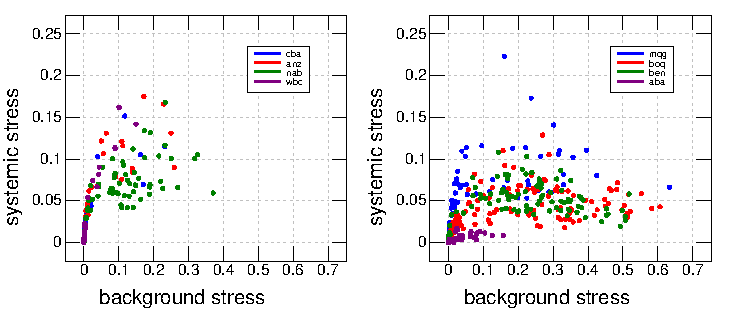
\includegraphics[width=12cm]{figures/sysstress.pdf}
\caption{\pr\  (y--axis) versus \br\  (x--axis)   for major banks (left panel) and  minor banks (right panel)  for 144 months during 2003--2014}
\label{sysstress}
\end{center}
\end{figure}

\subsection{Temporal \br\ in individual banks over time}\label{simulate1}

\fref{tbrisk} displays, the estimated $\br(S_i^+)$   for each major (left) and minor (right) Australian banks based on the projected one month ahead return distribution fitted using the GARCH--DCC model.   These \br\ results are discussed in \sref{brisk}.

\begin{figure}[htbp]
\begin{center}
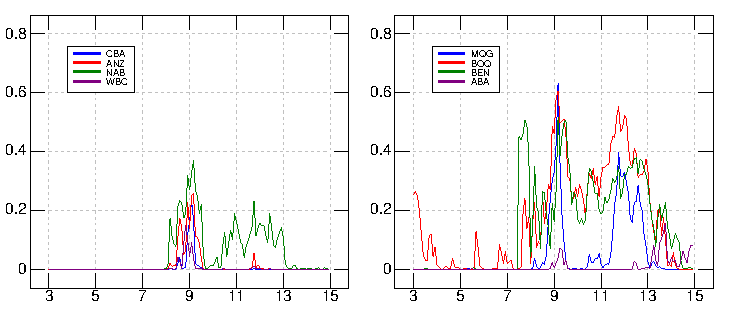
\includegraphics[width=12cm]{figures/tbrisk.pdf}
\caption{$\br(S_i^*)$  for   major (left panel) and  minor (right panel)  banks 2003--2014.}\label{tbrisk}
\end{center}
\end{figure}

\subsection{Temporal \pr\ in individual banks }

The panels in \fref{tprisk} show \pr\ computed by assuming the worst market return in 12 identical months. The \pr\ for each bank generally exhibits similar patterns as \br\ displayed in \fref{tbrisk}.  However the scale of \pr\ is  lower indicating bank return volatility is a more significant issue than the consequences of a major market downturn.  However, importantly, there are differing patterns of \pr\ across banks which is an important for the regulator. For example ANZ had similar \pr\ stress as NAB around 2012 but lower \br. Hence although ANZ was not obviously in stress during 2012, it would be if a market downturn occurred. BEN and BOQ had high \br\ levels after 2008, but are overtaken by MQG in terms of \pr: MQG is more likely to suffer in a market downturn whereas BEN and BOQ are less likely to be impacted.

\begin{figure}[htbp]
\begin{center}
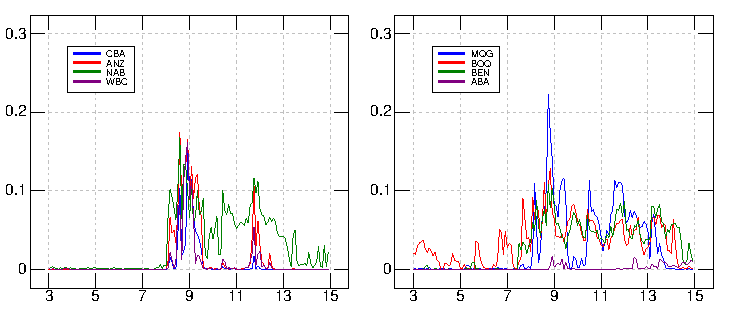
\includegraphics[width=12cm]{figures/tprisk.pdf}
\caption{$\pr(S_i^*)$  for   major (left panel) and  minor (right panel)  banks 2003--2014.}\label{tprisk}
\end{center}
\end{figure}

The above remarks are gleaned from the past behaviour of \pr\ over time.   In practice \pr\ and  \br\  will be monitored in real time providing up--to--date understanding of banks' risk positions as events unfold.   


\subsection{Temporal \br\  in the banking system}\label{Baggregate}

BRISK for both $S^*$ and $S^+$ are plotted in \fref{muqsB}.  With the former quantity risk is not diversified across banks.   The right panel indicates that initial build up of  $\br(S^*)$ is not immediately followed up by a build up of $\br(S^+)$: that is initially most \br\ is diversifiable.   However once a critical point is reached (at about 0.75) there is an almost linear progression and every unit increase in $\br(S^*)$ is transmitted to a unit increase in $\br(S^+)$, that is there is no more diversification or capacity to absorb \br.

\begin{figure}[htbp]
\begin{center}
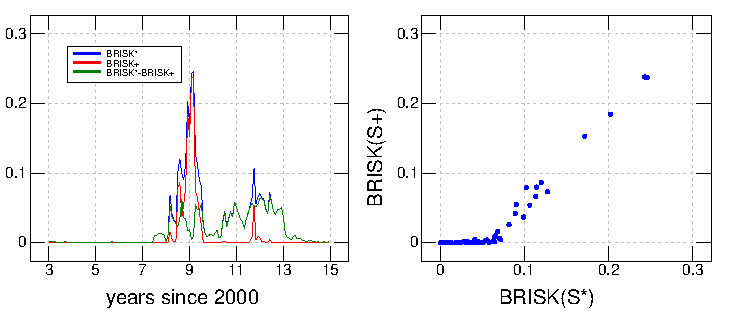
\includegraphics[width=12cm]{figures/muqsB.pdf}
\caption{$\br(S^*)$ and $\br(S^+)$ over time (left panel) and plotted against each other (right panel).}\label{muqsB}
\end{center}
\end{figure}

The capacity to absorb risk in the banking system relies on implicit merging and hence on a measure of shortfall such as $S^*$.    When two firms merge the leverage of the resulting firm is less than that of the more highly leveraged firm.   The merged firm is more able to withstand return on equity shocks  unless negative shocks are more prone for the merged firm.   

Firms do not necessarily merge, even in dire financial circumstances.   Hence the mergers spoken of here are hypothetical.   From a regulators perspective, what would happen under a merger of all firms (or perhaps a group of firms) is nevertheless of interest.   A system as as a whole near Basel breach is more threatening that one where a few firms are near Basel breach but the system as a whole is strongly Basel compliant.

\subsection{Temporal \pr\  in the banking system}\label{Paggregate}

PRISK for both $S^*$ and $S^+$ are plotted in \fref{muqsP}.  The scales are the same as in \fref{muqsB} facilitating comparison.   Note firstly \pr\ is generally smaller: that is systemic stress as induced by a major market event is generally smaller than stress caused by increases in volatility.   

Second, unlike baseline risk,   $\pr(S^+)$ can exceed $\pr(S^*)$ and in fact this occurs is quite typical in high stress environments.   Thus systemic risk in an aggregated system can be, and often is, higher than systemic risk in a disaggregated system suggesting interacting and reenforcing vulnerabilities. 

Third, the manner in which $\pr(S^+)$ builds up as compared to $\pr(S^*)$ is different to the buildup in \br.   This is evident in the right panel of \fref{muqsP}.  Low levels of $\pr(S^*)$ are not reflected in $\pr(S^+)$, that is all risk is absorbable in the system.   However once a critical level of $\pr(S^*)$ is reached there is an ``explosive" effect on the system as measured with $\pr(S^+)$: each unit increase in the former leads to a significantly higher than unit response in the latter.    

\begin{figure}[htbp]
\begin{center}
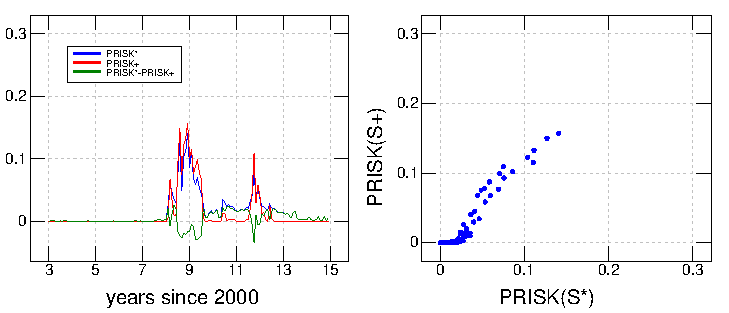
\includegraphics[width=12cm]{figures/muqsP.pdf}
\caption{$\pr(S^*)$ and $\pr(S^+)$ over time (left panel) and plotted against each other (right panel).}\label{muqsP}
\end{center}
\end{figure}




\section{Practical issues}\label{s_concl}

The following discusses key practical issues and challenges when calculating and monitoring baseline and systemic risks across firms. Performing the risk calculations requires a stochastic model which captures:
\begin{enumerate}
\i Future movements in firm balance sheets

\i Interdependence between firm balance sheets
\end{enumerate}
Modelling is a challenge given the complexity of firm balance sheets which are driven by a range of macroeconomic and firm specific factors. There are two approaches to the modelling: centralised or embedded in firm internal models. The centralised approach is discussed in this paper, using publicly available stock returns and making simplified assumptions on capital requirements, debt, and market returns being the driver of firm stock returns. The second approach of embedding the calculations in firm internal models is discussed below in this section.

The GARCH--DCC model proposed in this paper can be refined by identifying key items forming the balance sheet and their drivers apart from market returns. These drivers may include interest rates and potentially the entire yield curve, unemployment rates, GDP growth, and property prices (both residential and commercial). The impact of each driver differs by firm depending on the makeup of the balance sheet. For example a bank balance sheet where assets are mainly formed by residential loans will be more sensitive to residential property prices than another which is mainly formed by commercial loans. Analysing balance sheets and drivers in detail leads to refinements in modelling and baseline and systemic risk calculations.

Once a centralised model is built, data and calculations need to be continually refreshed to monitor baseline and systemic risks over time. This ensures that risk calculations are reflective of current levels of debt, leverage, volatility and correlation. The continual updating requires a tradeoff between model sophistication and the effort required to perform the calculations. A sophisticated model may produce accurate risk calculations at a certain point in time, but may require significant time and resources to refresh calculations on say a daily or even monthly basis. In this case a simpler model may be more suitable without significantly comprising the quality of the results.


It is likely that firms have sophisticated stochastic models of their balance sheets, and hence baseline and systemic risk calculations may be embedded in these models. For example banks which are accredited to use the Internal Ratings Based (IRB) approach and Advanced Measurement Approach (AMA) to calculate their regulatory capital requirements will have advanced stochastic models of their balance sheet over at least a one year. However given that the models are proprietary, a key challenge would be to access and integrate models across firms, and continually over time. Even if the models are available, they may be inconsistent (for example using different time intervals or macroeconomic drivers) which makes the integration challenging. The challenge increases when systemic risk is expanded to capture banking and insurance industries.

A more practical alternative is to rely on individual firms to perform calculations of their baseline and systemic risks, similar to how Australian banks were made to perform industry stress tests in 2014 and prior. Consistency in the calculations would be the main focus, and could be improved by for example supplying a common ESG (Economic Scenario Generator) to all firms although the practicality of doing so has to be assessed. In addition a frequent additional stress test exercise may be onerous for firms.




\newpage





\appendix
\renewcommand*{\thesection}{\Alph{section}}

\section{GARCH--DCC model}\label{garchdcc}

Denote the daily (log) return for firm $i$ at time $t$ as
\newcommand{\vareps}{\varepsilon}
\be{mean.model}
\delta_{it}=\mu_i+\sigma_{it}\eps_{it}\cq \eps_{it}\sim (0,1)\ .
\ee
The volatility $\sigma_{it}$ is modelled as
\be{vol}
\sigma_{i,t+1}^2 = \omega+ \sigma^2_{it}\{\beta+(\alpha+\gamma \eps^-_{it})\eps_{it}^2\}  \cq  \eps^-_{it}\equiv I(\eps_{it}<0)=I(\delta_{it}<\mu)\ ,
\ee
where $I$ denotes the indicator function.  Hence the response of $\sigma_{i,t+1}^2$ to $\eps_{it}^2$  is increased by $\gamma$   if
the rate of return is below the average $\mu_i$, compared to the response if $\delta_{it}>\mu_i$.  Equations \eref{mean.model} and \eref{vol} defined a simple threshold GARCH model:  called the TARCH(1,1).   In \eref{mean.model} the mean $\mu_i$ does not vary with time $t$ and in \eref{vol} it is assumed the terms  $\sigma_{it}^2$ and $\eps_{it}$ in the right hand side of \eref{vol} are sufficient to structure the dynamics of volatility and contemporaneous correlation.

The model defined by \eref{mean.model} and \eref{vol} is estimated  for each security $i$ jointly with  a similar model for  the market,  $i=m$.   Correlation between security $i$ and the market $m$ are implicitly modelled using  positive definite recursions   \citep{engle2002dynamic}
$$
(Q_{i,t+1}-S) = \alpha (\eta_{it}\eta_{it}'-S) + \beta (Q_{it}-S)\cq \eta_{it}\equiv(\eps_{it},\eps_{mt})' .
$$
The correlation defined by $Q_{it}$ is used as the correlation between $\eps_{it}$ and $\eps_{mt}$.


\section{Data sources}\label{data}

Data are sourced from DataStream using the company and datatype codes as set out in \tref{datastream}.

\begin{table}\caption{DataStream codes}\label{datastream}
\begin{center}
	\begin{tabular}{l|l}
	\hline
	\multicolumn{2}{l}{Company codes}\\
	\hline
A:ANZX & Australia and New Zealand Banking Group Limited\\
A:ABAX & Auswide Bank Limited\\
A:BOQX & Bank of Queensland Limited\\
A:BENX & Bendigo and Adelaide Bank Limited\\
A:CBAX & Commonwealth Bank of Australia\\
A:MQGX & Macquarie Bank Limited\\
A:NABX & National Australia Bank Limited\\
A:WBCX & Westpac Banking Corporation.\\
\hline
\multicolumn{2}{l}{Datatype codes}\\
\hline
	NOSH & Number of Shares\\
	P & Price\\
	WC02999 & Total Assets\\
	WC03501 & Shareholders Equity\\
	RZ & Total return index\\
\hline	
\end{tabular}
\end{center}
\end{table}

Firm equity $w$ is Number of Shares multiplied by Price. Firm debt $d$ is Total Assets minus Shareholders Equity. Stock returns are computed from the Total Return Index including paid dividends. 

\newpage
\section{References}
\bibliography{piet2}


\end{document}

